\documentclass{article}

\usepackage{polski}
\usepackage[utf8]{inputenc}
\usepackage{graphicx}
\usepackage{float}
\usepackage{listings}
\usepackage{graphicx}
\renewcommand{\lstlistingname}{Funkcja}
\renewcommand{\theparagraph}{\alph{paragraph}) }\setcounter{secnumdepth}{4}
\lstset{language=C++,
numbers=left}


\author{Dominik Doberski, Artur Olejnik}
\title{
\huge Sprawozdanie 
\\Przetwarzanie równoległe\\
\Huge Projekt 1 OMP}



\begin{document}
\maketitle

\section{Wstęp}
\subsection{Temat}
Mnożenie macierzy - porównanie efektywności metod --
\begin{itemize}
\item 3 pętle - kolejność pętli: jik, podział pracy przed pętlą 1
\item 6 pętli -kolejność pętli: zewnętrznych ijk, wewnętrznych: ii,kk,jj podział pracy przed pętlą 2.
\end{itemize}
\subsection{Autorzy}
\begin{minipage}[t]{0.3\textwidth}
% Pierwsza kolumna (średnia)
Dominik Doberski\\
Artur Olejnik
\end{minipage}
\begin{minipage}[t]{0.15\textwidth}
% Druga kolumna (mniejsza)
132207\\
122402
\end{minipage}
\begin{minipage}[t]{0.55\textwidth}
% Trzecia kolumna (mniejsza)
dominik.doberski@student.put.poznan.pl\\
artur.olejnik@student.put.poznan.pl
\end{minipage}
\\\\\\
Grupa dziekańska I3\\
Termin zajęć: poniedziałek 16:50 
\subsection{Opis systemu obliczeniowego}
Do wykonania pomiarów wykorzystano program CodeXL. Testy zrealizowano na jednostce obliczeniowej o poniższej specyfikacji:
\begin{itemize}
\item Nazwa: AMD FX-6300
\item Częstotliwość taktowania: 3.5 GHz (max 3.8 GHz)
\item Liczba procesorów fizycznych: 3
\item Liczba procesorów logicznych: 6
\item Liczba uruchamianych w systemie wątków: 6
\item Wielkość i organizacja pamięci podręcznych procesora:\\
L1 dane: 6x16KB\\
L1 instrukcje: 3x64KB\\
L2: 3x2MB\\
L3: 8MB\\
\end{itemize}

\section{Analiza algorytmu}
\subsection{Kluczowe fragmenty kodu}
\begin{lstlisting}[
caption={3 pętle -- jik},
label=1. funkcja,
firstnumber=1]
void multiply_matrices_JIK() {
#pragma omp parallel
#pragma omp for 
 for (int j = 0; j < ROWS; j++){
  for (int i = 0; i < ROWS; i++){
   for (int k = 0; k < ROWS; k++){
    matrix_r[i][j] += matrix_a[i][k] * matrix_b[k][j];
   }}}}
\end{lstlisting}

W powyższej funkcji pętla w 6. wierszu iteruje po kolumnach macierzy $A$ i po wierszach macierzy $B$. Iloczyn tych dwóch elementów jest dodawany do pojedynczego elementu macierzy $R$ znajdującego się w $i$-tym wierszu i $j$-tej kolumnie, które są wyznaczane w pętlach odpowiednio 5. i 4. wierszu. Złożoność algorytmu wynosi $O(n^3)$.

\begin{figure}[H]
	\centering
	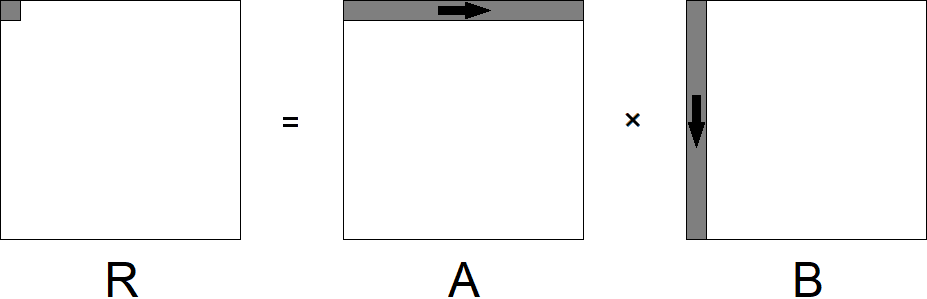
\includegraphics[bb=0 0 1280 960]{./images/3/lokIn.png}
	\caption{Zasoby wykorzystywane w pętli wewnętrznej}
	\label{fig:3inner}
\end{figure}

Powyższy rysunek przedstawia dokładnie, które dane są wykorzystywane do przetworzenia pętli w 6. linii kodu. Jak widać do wykonania jednej iteracji pętli wewnętrznej potrzebne jest odczytanie jednego wiersza macierzy A i jednej kolumny macierzy B. Rezultatem tej pętli będzie odczytanie jednej wartości macierzy wynikowej R.

\begin{figure}[H]
	\centering
	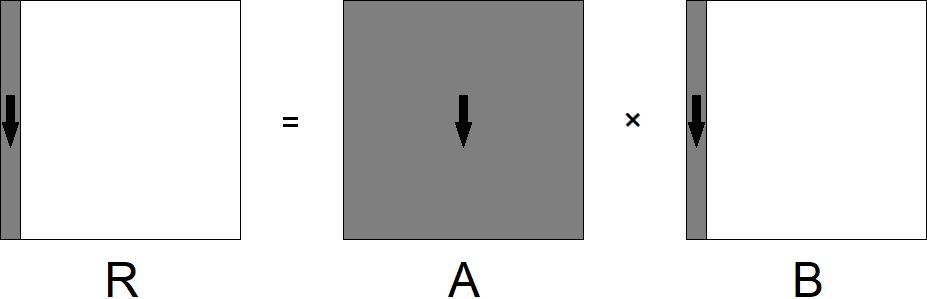
\includegraphics[bb=0 0 1280 960]{./images/3/lokMed.png}
	\caption{Zasoby wykorzystywane w pętli środkowej}
	\label{fig:3medium}
\end{figure}

Drugi rysunek ilustruje wykorzystanie danych do zrealizowania pętli w 5. wierszu. W tym przypadku potrzeba już wszystkich danych z macierzy A i, tak jak w przypadku samej pętli wewnętrznej, jednej kolumny macierzy B. Otrzymujemy całą kolumnę macierzy wynikowej R. Wykonanie pętli zewnętrznej pozwoli na uzyskanie wartości wszystkich kolumn macierzy R.

Dyrektywy OpenMP w 2. i 3. wierszu wykorzystano do uruchomienia kodu na wielu wątkach oraz podzielenia przetwarzania pętli między nimi. Kolejne iteracje pętli w 4. wierszu zostaną przydzielone równomiernie między wątki. Spowoduje to, że kolumny macierzy $B$ i macierzy wynikowej $R$ nie będą się powtarzały w kolejnych wątkach.

\begin{lstlisting}[
caption={6 pętli -- zewnętrzne ijk, wewnętrzne ii,kk,jj},
label=2. funkcja,
firstnumber=9]
void multiply_matrices_6(int r){
#pragma omp parallel
 for (int i = 0; i < ROWS; i += r) {
#pragma omp for
  for (int j = 0; j < ROWS; j += r) {
   for (int k = 0; k < ROWS; k += r) {
    for (int ii = i; ii < i + r; ii++) {
     for (int kk = k; kk < k + r; kk++) {
      for (int jj = j; jj < j + r; jj++) {
       matrix_r[ii][jj] += matrix_a[ii][kk] * matrix_b[kk][jj];
      }}}}}}}
\end{lstlisting}

Druga funkcja jest bardziej złożona. 3 wewnętrzne pętle pracują podobnie jak pętle w poprzedniej funkcji, ale pracują tylko dla określonego fragmentu każdej z tych macierzy. Wielkość tego obszaru jest określona w argumencie $r$. Pętla w 14. wierszu sumuje wartości komórek otrzymanego fragmentu z iloczynami innych potrzebnych fragmentów. Pętle w 11. i 13. wierszu iterują po każdym fragmencie w celu wyliczenia wartości każdej komórki macierzy wynikowej $R$. Złożoność tego rozwiązania wynosi $O((\frac{n}{r})^3*r^3)=O(n^3)$.

Dyrektywy OpenMP działają podobnie jak w pierwszej funkcji. Tutaj pomiędzy wątki równomiernie zostają rozdzielone kolejne iteracje pętli w 13. wierszu.

\subsection{Analiza efektywności}
\subsubsection{Podział pracy na wątki}

W pierwszej funkcji wątek dokonuje obliczeń dla pojedynczej kolumny macierzy wynikowej $R$. Wykorzystuje do tego jedną kolumnę macierzy $B$ i całą macierz~$B$. Dla drugiej funkcji zrównoleglenie odbywa się dla pętli w 13. wierszu, a więc wątki również dokonują obliczeń dla kolumn macierzy wynikowej $R$. Różnica polega na tym, że w tym przypadku obliczenia są dokonywane nie dla jednej kolumny, a dla grupy $r$ kolumn, gdzie $r$ jest argumentem tej funkcji.

\subsubsection{False sharing}

Z powyższych rozważań wynika, że w obu funkcjach każdy wątek w jednej chwili oblicza inny fragment macierzy wynikowej $R$. Nie będzie zatem potrzebne synchronizowanie pracy różnych wątków i nie dojdzie do unieważnienia danych -- false sharing nie zachodzi.

\subsubsection{Analiza lokalności dostępu do danych}

Rozróżniamy dwa rodzaje lokalności -- czasową i przestrzenną. Pierwsza oznacza wielokrotne odwoływanie się wątków do danych przetrzymywanych w pamięci podręcznej. Do jej wystąpienia wymagane jest odpowiednio duży rozmiar pamięci podręcznej, która musi być większa od rozmiaru pamięci potrzebnej do wykonania danej operacji. Lokalność przestrzenna polega na dostępie do danych występujących jeden po drugim w pobranej linii pamięci czyli w jednym wierszu macierzy.

W poniższych punktach przeprowadziliśmy analizę pod względem występowania lokalności dla różnych rozmieszczeń dyrektywy \textit{\#pragma omp for}.

\paragraph{Lokalność dla pierwszej funkcji}

\begin{itemize}
\item Przed pętlą w 4. linii kodu


Powyższy rysunek przedstawia, które elementy każdej z 3 macierzy są brane pod uwagę w pętli zewnętrznej. 

\item Przed pętlą w 5. linii kodu
\end{itemize}

\paragraph{Lokalność dla drugiej funkcji}


\section{Analiza przetwarzania}
\subsection{Przebieg}
Instancja graniczna

Dla danego problemu istnieje instancja graniczna, ze względu na ograniczoną pojemność pamięci podręcznej L3. Zastosowana pamięć L3 w procesorze ma pojemność 8 MB. Przekroczenie pojemności tej pamięci powoduje znaczne spowolnienie działania algorytmu. Zmiennych typu float (rozmiar 4B) na których przeprowadzane są obliczenia, możemy przechować: 
\[ 8MB/4B = 2 * 1024 * 1024 = 2097152 \]
Pamięć L3 jest współdzielona przez wszystkie rdzenie procesora, więc dane które nie mieszczą się w L3, muszą zostać przeniesione do pamięci RAM, co powoduje zwiększenie czasu przetwarzania.

W wersji algorytmu 3 pętlowej, każdy wątek musi załadować do pamięci kolumnę macierzy wynikowej R, całą macierz A oraz kolumnę macierzy B.
Należy zatem posłużyć się wzorem:
\[ n_R + n_A^2 + n_B < 2097152 \]

Wynikiem jest:
\[ n_R = n_A = n_B = 1447\]

Eksperyment zostanie przeprowadzony na dwóch rozmiarach instancji: 1400,  1500 oraz 1600.


\subsection{Wyniki}
Instruction per Cycle (IPC) - stosunek wykonanych istrukcji i liczby cykli zegara, im większa jest to wartość, tym więcej wykonujemy instrukcji na cykl, a więc wykorzystanie procesora jest lepsze.

\begin{figure}[H]
	\centering
	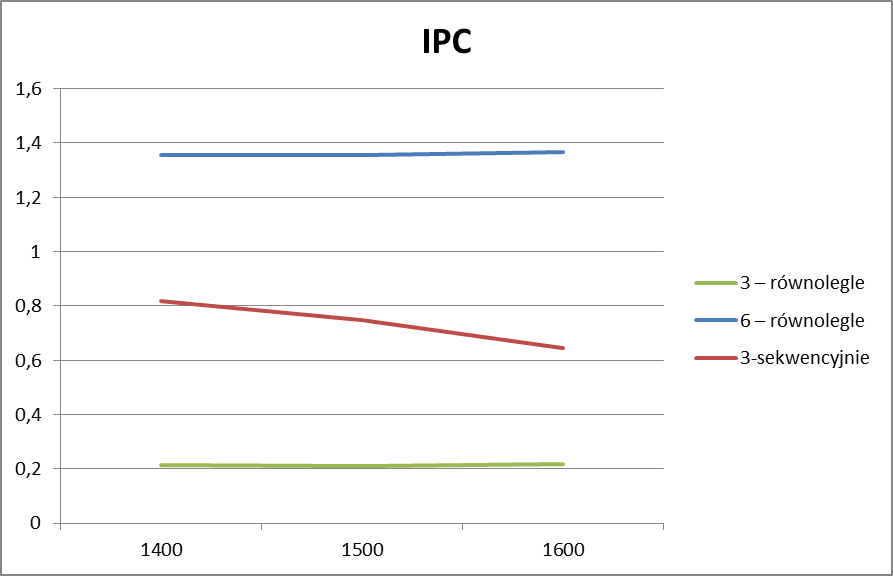
\includegraphics[bb=0 0 1280 960]{./images/wykresy/IPC.png}
	\caption{Zasoby wykorzystywane w pętli środkowej}
	\label{fig:3medium}
\end{figure}

Data cache miss ratio - stosunek nietrafień do pamięci podręcznej i wszystkich dostępów zrealizowanych. Im mniejszy jest ten wynik, tym rzadziej trzeba odwoływać się dalej, niż do pamięci podręcznej. 

\begin{figure}[H]
	\centering
	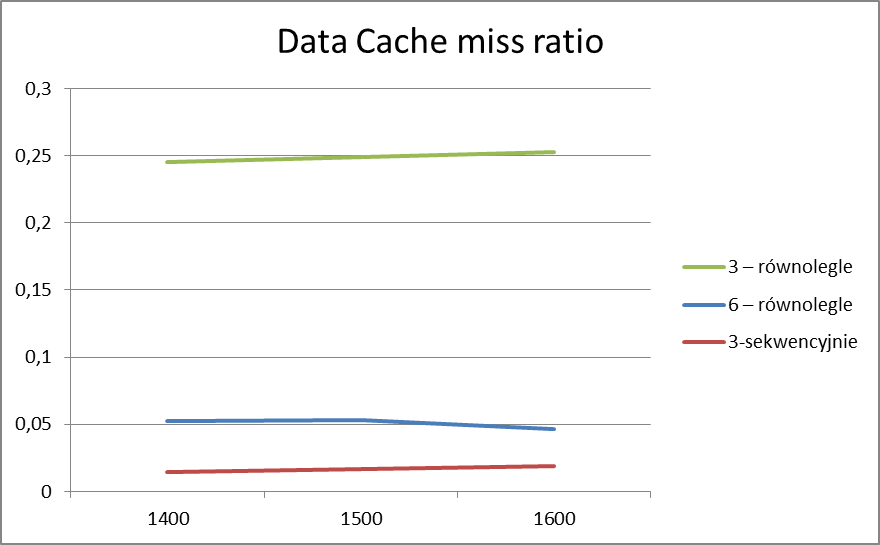
\includegraphics[bb=0 0 1280 960]{./images/wykresy/Data Cache miss ratio.png}
	\caption{Zasoby wykorzystywane w pętli środkowej}
	\label{fig:3medium}
\end{figure}

Data cache miss rate - stosunek nietrafień do pamięci podręcznej i wykonanych instrukcji. Im większa jest ta wartość, tym wolniej realizowane jest przetwarzanie.  

\begin{figure}[H]
	\centering
	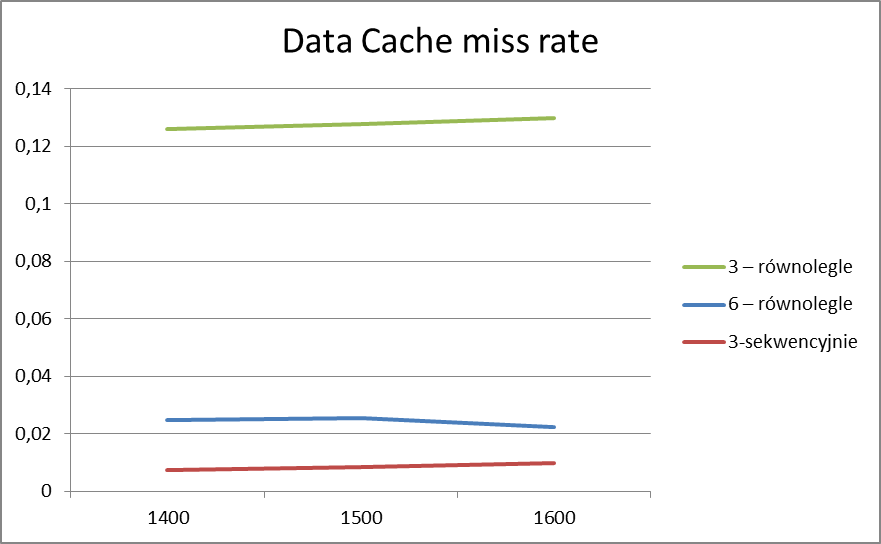
\includegraphics[bb=0 0 1280 960]{./images/wykresy/Data Cache miss rate.png}
	\caption{Zasoby wykorzystywane w pętli środkowej}
	\label{fig:3medium}
\end{figure}



\subsection{Prezentacja wzorców}
asdf
\subsection{Miary przetwarzania}
asdf

\section{Wnioski}
Data Cache miss ratio - jest to stosunek nietrafień do pamięci podręcznej do dostępów zrealizowanych.


\subsection{Wypunktowania}
To jest wypunktowanie:
\begin{itemize}
\item punkt
\item punkt
\item punkt
\end{itemize}
\subsection{Wyliczenie}
To jest wyliczenie:
\begin{enumerate}
\item pierwszy,
\item drugi,
\item trzeci.
\end{enumerate}
\subsection{Wykres}
Na Rysunku~\ref{fig:wykres} znajduje się przykładowy wykres.
\subsection{Wzory}
\begin{equation}
2 + 2 = 4
\end{equation}
\begin{equation}
E = mc^2
\end{equation}
\begin{equation}
\left[- \frac{\hbar^2}{2M} + V(X) \right] \Psi(x)=  \mathcal{E} \Psi(x)
\end{equation}

\section{Podsumowanie}

\end{document}
